\documentclass[letterpaper,final,12pt,reqno]{amsart}

\usepackage[total={6.3in,9.2in},top=1.1in,left=1.1in]{geometry}

\usepackage{times,bm,bbm,empheq,fancyvrb,graphicx}
\usepackage[dvipsnames]{xcolor}
\usepackage{tikz}
\usetikzlibrary{decorations.pathreplacing}

\usepackage[kw]{pseudo}
\pseudoset{left-margin=15mm,topsep=5mm,idfont=\texttt}

% hyperref should be the last package we load
\usepackage[pdftex,
colorlinks=true,
plainpages=false, % only if colorlinks=true
linkcolor=blue,   % ...
citecolor=Red,    % ...
urlcolor=black    % ...
]{hyperref}

\renewcommand{\baselinestretch}{1.05}

\newtheorem{lemma}{Lemma}

\newcommand{\Matlab}{\textsc{Matlab}\xspace}
\newcommand{\eps}{\epsilon}
\newcommand{\RR}{\mathbb{R}}

\newcommand{\grad}{\nabla}
\newcommand{\Div}{\nabla\cdot}
\newcommand{\trace}{\operatorname{tr}}

\newcommand{\hbn}{\hat{\mathbf{n}}}

\newcommand{\bb}{\mathbf{b}}
\newcommand{\bbf}{\mathbf{f}}
\newcommand{\bg}{\mathbf{g}}
\newcommand{\bn}{\mathbf{n}}
\newcommand{\bu}{\mathbf{u}}
\newcommand{\bv}{\mathbf{v}}
\newcommand{\bw}{\mathbf{w}}
\newcommand{\bx}{\mathbf{x}}

\newcommand{\bV}{\mathbf{V}}
\newcommand{\bX}{\mathbf{X}}

\newcommand{\bxi}{\bm{\xi}}

\newcommand{\bzero}{\bm{0}}

\newcommand{\rhoi}{\rho_{\text{i}}}

\newcommand{\ip}[2]{\left<#1,#2\right>}


\begin{document}
\title[Geometric multigrid for glacier modeling]{Geometric multigrid for glacier modeling: \\ A user's guide}

\author{Ed Bueler}

\begin{abstract} FIXME: two principles in introduction: mass conservation complementarity, solver optimality.  four examples in sections \ref{sec:subspace}--\ref{sec:stokes}: poisson equation from subspace decomp point of view, obstacle problem by subset decomposition, monotone multigrid for implicitly-evolving SIA geometry, Schur-complement and Vanka Newton-multigrid for fixed-geometry Glen-Stokes
\end{abstract}

\maketitle

\tableofcontents

\thispagestyle{empty}
\bigskip

\section{Introduction} \label{sec:intro}

The construction of effective numerical glacier and ice sheet models is challenging for two fundamental reasons.  First is the complexity of the equations and boundary conditions.  Indeed, the physics of glaciers is nonlinear, nontrivially-coupled, and subject to imperfectly-understood boundary processes, such as at contact with ocean water.  The coupling is critical in the sense that mass, momentum, and energy conservation interact in ways which are relevant to glaciological modeling goals, such as when basal sliding, and thus ice velocity, is only determined though a simultaneous momentum and energy solution.  Second, the geometry of glaciers and ice sheets is complex, and in particular the fastest-flowing parts of ice sheets are often located at the geometrically-nontrivial lateral boundary where fjord-like bed geometry is also common.  Numerical models therefore need to perform expensive fine-mesh calculations, so as to accomodate the complicated, changing boundary geometry, while solving relatively-complicated multiphysics equations.

On the other hand, since the 1980s researchers in numerial methods have developed multigrid methods to solve partial differential equations like those which describe the ice fluid in glaciers.   For simpler problems like scalar elliptic equations and the linear Stokes system, especially on domains which have a simpler geometry, these methods are now in routine use \cite{Briggsetal2000,Bueler2021,Trottenbergetal2001}.

FIXME perspectives \emph{not} found here: convergence of GMG (or much detail for application to linear problems); assumptions like ``SPD'' specific to constrained \emph{optimization} as opposed to VI/NCP viewpoint


\section{From subspace decomposition to multigrid (for the Poisson equation)} \label{sec:subspace}

In this section we will demonstrate how to solve a simple ordinary differential equation (ODE), namely the Poisson problem
\begin{equation}
- u''(x) = f(x) \quad \text{on} \quad 0 \le x \le 1, \label{eq:poisson}
\end{equation}
with Dirichlet boundary conditions $u(0)=u(1)=0$, using a finite element (FE) discretization and a simple multigrid method.  Over the course of this and the next two sections, this simple equation will ``evolve'' into a realistic model for glacier geometry.

Our numerical approximation of \eqref{eq:poisson} uses an unequally-spaced mesh of $m$ interior \emph{nodes} (points) $x_p$ on $(0,1)$, and the open intervals between the nodes are the $m+1$ \emph{elements}.  The numerical solution $u^h(x)$ is a linear combination of the piecewise-linear hat functions $\psi_p(x)$, shown in Figure \ref{fig:finehats}, one for each interior node:
\begin{equation}
u^h(x) = \sum_{p=1}^m u_p \psi_p(x). \label{eq:trialsolution}
\end{equation}
Each hat function $\psi_p(x)$ is defined on all of $[0,1]$, satisfies $\psi_p(x_q) = \delta_{pq}$, is linear on the elements, and is continuous.  The set $\{\psi_p(x)\}_{p=1}^m$ is a \emph{nodal basis} of the space $\mathcal{V}^h$ of continuous, piecewise-linear functions in the sense that the coefficients are the function values: $u_p=u^h(x_p)$.  Note that the derivative of $u^h(x)$ is defined on the elements, but not generally at the nodes.

\begin{figure}
\includegraphics[width=0.65\textwidth]{figs/finehats.pdf}
\caption{Hat functions $\psi_p(x)$ at interior points $x_p$ form a basis for the vector space $\mathcal{V}^h$ of piecewise-linear functions  with zero boundary values.}
\label{fig:finehats}
\end{figure}

Having represented the solution, to actually solve the problem we must adjust the coefficients $u_p$ to their correct values.  In a program these coefficients are formed into a column vector $\bu=\{u_p\}$ in $\RR^m$.  We will approximate equation \eqref{eq:poisson} so as to construct a linear system to determine $\bu$.  Our applications of multigrid ideas to glacier problems will be clearest if we adopt a finite element (FE) approach based on re-phrasing \eqref{eq:poisson} in \emph{weak form} using integrals.  Accessible introductions to FE methods are in \cite{Bueler2021,Elmanetal2014,Johnson2009}.  Note that once we state the weak form then the original equation will be called the \emph{strong form}.

The weak form of \eqref{eq:poisson} arises by multiplying both sides of the equation by a \emph{test function} and integrating by parts so that only first derivatives remain.  Without committing to any mathematical detail, we suppose the exact, continuum solution $u(x)$ comes from a vector space $\mathcal{H}$ of functions which are smooth enough to allow the computations which follow and which have value zero at $x=0$ and $x=1$.  Choosing a test function $v(x)$ also from $\mathcal{H}$, by multiplying both sides of \eqref{eq:poisson} by $v$ and integrating by parts, and by using $v(0)=v(1)=0$, we find
\begin{equation}
\int_0^1 u'(x) v'(x)\,dx = \int_0^1 f(x) v(x)\, dx.  \label{eq:weakpoissonearly}
\end{equation}
We write equation \eqref{eq:weakpoissonearly} more compactly as
\begin{equation}
  a(u,v) = \ip{f}{v} \label{eq:weakpoisson}
\end{equation}
defining each side as in \eqref{eq:weakpoissonearly}.  The reasons for this notational simplification will become clear as we describe multigrid algorithms.  For $u,v$ in $\mathcal{H}$, the left side $a(u,v)$ is linear in each argument (\emph{bilinear}) while the right side defines a \emph{linear functional} $\ell[v] = \ip{f}{v}$.

One may now substitute the \emph{trial} formula \eqref{eq:trialsolution} for $u^h$ into \eqref{eq:weakpoisson} to derive a linear system
\begin{equation}
A \bu = \bbf, \label{eq:linearsystem}
\end{equation}
where $A$ is an $m\times m$ matrix and $\bbf$ is in $\RR^m$.  Note that each equation in system \eqref{eq:linearsystem} is constructed by using a hat function as a test function; substitution of $v=\psi_p$ into \eqref{eq:weakpoisson} gives the $p$th equation in \eqref{eq:linearsystem}.  The symmetric matrix $A$, which is positive definite for this Poisson equation \cite{Elmanetal2014}, has entries $a_{pq} = a(\psi_p,\psi_q)$.  For the right side one defines $f_p = \ip{f}{\psi_p} = \ell[\psi_p]$ to form the vector $\bbf = \{f_p\}$.

The most straightforward way to ask a computer to solve the assembled linear system \eqref{eq:linearsystem} would be by a direct method such as Gaussian elimination.  However, in higher-dimensional PDE problems such methods need much more that $O(m)$ operations to solve the system.  As noted in the introduction, large-scale applications need optimal $O(m)$ solution methods, or nearly so, thus our focus on multigrid.  Furthermore, after this section all of our problems will be nonlinear, thus no direct method will be available, and indeed we will generally not assemble matrix objects at all.  Instead we will need rapidly-convergent iterations for our finite-dimensional and nonlinear FE systems for glacier problems.

On the basis of the above simple FE scheme we now take the first step to build a \emph{multilevel} or multigrid scheme.  Consider an enlarged set of hat functions:
    $$\underbrace{\psi_1(x),\dots,\psi_m(x)}_{\text{existing fine level}},\underbrace{\psi_{m+1}(x),\dots,\psi_M(x)}_{\text{coarser levels}}$$
For example, two coarser levels are shown in Figure \ref{fig:coarsehats}, based on the fine level in Figure \ref{fig:finehats}.  The first coarsening (top of Figure \ref{fig:coarsehats}) comes from by-passing every other node on the fine mesh, and the next coarsening (bottom) does this again.  (On 2D and 3D meshes this manner of constructing coarse-mesh hats is much less straightforward, and it is more common to start from a coarse mesh and refine level-by-level up to the fine level.)  One may regard the coarsening process as the selection of coarse-mesh nodes, but the hat functions on the coarse level, once identified, contain the information needed to do coarse-level calculations.

\begin{figure}
\includegraphics[width=0.55\textwidth]{figs/coarsehats.pdf}
\smallskip

\includegraphics[width=0.55\textwidth]{figs/coarsesthats.pdf}
\caption{In our FE method the coarser levels are simply additional sets of hat functions which spread over a greater distance.}
\label{fig:coarsehats}
\end{figure}

We need notation for the levels.  Suppose that the coarsest is indexed as $k=0$ and the finest as $k=K$, with intermediate levels $k=1,\dots,K-1$, so
\begin{equation}
  \psi_j^k(x) \quad \text{for } j=1,\dots,m_k \text{ form the $k$th level},  \label{eq:definepsijk}
\end{equation}
and the interior nodes $x_j^k$ use the same indexing scheme.  Note the fine level has now gained a superscript $K$, thus the original hats are now $\psi_j^K(x)$ and the nodes are $x_j^K$.  For example, Figures \ref{fig:finehats} and \ref{fig:coarsehats} show a three-level scheme ($K=2$) with a total of $m_2=11$ interior nodes.  There are $m_1=5$ intermediate level hats and $m_0=2$ coarsest-level hats.  The original mesh has $m_2+1=12$ elements, divisible by four, so the above coarsening scheme works.

The $k$th level in our multilevel scheme is really a vector space, namely
\begin{equation}
  \mathcal{V}^k = \operatorname{span}\{\psi_1^k(x),\dots,\psi_{m_k}^k(x)\}.  \label{eq:definevk}
\end{equation}
These hat functions are linearly-independent and form a basis for $\mathcal{V}^k$.  The dimension of $\mathcal{V}^k$ is $m_k$ and the dimension of the whole FE solution space $\mathcal{V}^h$, now also denoted $\mathcal{V}^K$, is $m_K$.  In fact these vector spaces are nested, $\mathcal{V}^{k-1} \subset \mathcal{V}^k$, because a coarser-level hat function can be written as a linear combination of next-finer hats:
\begin{equation}
   \psi_j^{k-1}(x) = \sum_{\ell=1}^{m_k} c_\ell \psi_\ell^k(x). \label{eq:hatcombination}
\end{equation}
The only nonzero coefficients $c_\ell$ are those where the support of $\psi_j^{k-1}(x)$ overlaps nontrivially with the support of $\psi_\ell^k(x)$.

The multilevel \emph{subspace decomposition} is described by a vector space sum:
\begin{equation}
  \mathcal{V}^h = \mathcal{V}^0 + \mathcal{V}^1 + \dots + \mathcal{V}^K. \label{eq:subspacedecomposition}
\end{equation}
This will be useful even though the final term $\mathcal{V}^K$ is actually equal to the whole space $\mathcal{V}^h$.  Equation \eqref{eq:subspacedecomposition} only asserts that a piecewise-linear function (i.e.~in $\mathcal{V}^h$) \emph{can} be written as a linear combination of hat functions from all the levels.  There is no unique representation.  Our multigrid method will use this hierarchy of levels to ultimately find the components of the solution in the fine-level space $\mathcal{V}^h=\mathcal{V}^K$, but via fast computations on all levels $\mathcal{V}^k$.  On each level we will reduce the energy of the current solution estimate (i.e.~iterate) in that space.

The coarser levels $\mathcal{V}^0,\dots,\mathcal{V}^{K-1}$ would seem not to add any value as they are mere subspaces of the fine-level space $\mathcal{V}^K$.  However, they provide a \emph{scale of frequencies}.  Informally, if $g(x)$ is any function on $[0,1]$ then the value of its inner product with a fine-level hat, $\ip{g}{\psi_j^K} = \int_0^1 g(x) \psi_j^K(x)\,dx$, relative to its norm $\|g\| = \ip{g}{g}^{1/2}$, is a measure of its high-frequency content at $x_j^K$.  The inner product with a coarse-mesh hat, by contrast, measures a lower frequency at that location.  (If decomposition \eqref{eq:subspacedecomposition} were a Fourier decomposition, with each $\mathcal{V}^k$ spanned by sines and cosines of disjoint ranges of frequencies, then the sum would be orthogonal and the ``scale of frequencies'' meaning would be exact.)

Recall the weak form \eqref{eq:weakpoisson}.  The goal of our FE method is to find a solution $u^K$ on the fine level $\mathcal{V}^K$ so that \eqref{eq:weakpoisson} holds for all test functions $v$ in $\mathcal{V}^K$.  It will be essential to treat the right-hand side abstractly, and on the fine level we define the linear functional
\begin{equation}
  \ell^K[v] = \ip{f}{v}.  \label{eq:rhsfine}
\end{equation}
On other mesh levels we will also have a right-hand-side linear functional $\ell^k[v]$ acting on $v$ in $\mathcal{V}^k$ (below), but defined by new formulae below.  In any case we solve a finite-dimensional weak-form equation on each level $k$,
\begin{equation}
  a(u^k,v) = \ell^k[v],  \label{eq:feweakpoisson}
\end{equation}
for all $v$ in $\mathcal{V}^k$, where the bilinear form $a(u,v)$ has the same meaning on each level, namely as the left side of \eqref{eq:weakpoissonearly}.  Our solution method does not need to assemble a matrix for system \eqref{eq:feweakpoisson}, while on the other hand it can be modified \eqref{eq:feweakpoisson} into an analogous weak form for the nonlinear and inequality-constrained glacier geometry problem in the next two sections \ref{sec:obstacle}, \ref{sec:sia}.

Suppose $w(x)$ in $\mathcal{V}^k$ is an approximation of the solution $u^k$.  Define the \emph{residual} as the linear functional
\begin{equation}
  r^k(w)[v] = \ell^k[v] - a(w,v)  \label{eq:residual}
\end{equation}
acting on $v$ in $\mathcal{V}^k$.  Clearly, finding $w$ such that $r^k(w)=0$ solves \eqref{eq:feweakpoisson}.

On each mesh level our only solution method for \eqref{eq:feweakpoisson} is \emph{Gauss-Seidel (GS) iteration}, namely sequential and point-wise \emph{relaxation}.  Though matrices are used to present the GS algorithm in many sources \cite[for example]{Bueler2021,Greenbaum1997}, there is no true need for such objects; we will present the algorithm using only the residual and the weak form.

The GS iteration sweeps goes through the level-$k$ hat functions $\psi_p^k$, modifying the iterate $w(x)$ by a multiple of $\psi_p^k$ so as to make $r^k(w)[\psi_p^k]=0$.  That is, it makes the residual zero at $x_p^k$.  By linearity of the form $a(\cdot,\cdot)$ in the first argument, if $w(x) = \sum_{q=1}^{m_k} w[q] \psi_q^k(x)$ then
\begin{equation}
  r^k(w)[\psi_p^k] = \ell^k[p] - \sum_{q=1}^{m_k} a(\psi_q^k,\psi_p^k)\, w[q].  \label{eq:residualpoisson}
\end{equation}
(Note $\ell^k[p] = \ell^k[\psi_p^k]$ by definition.)  The GS pointwise equation finds a real number $c$ so that
\begin{equation}
  r^k(w+c\,\psi_p^k)[\psi_p^k] = 0,  \label{eq:gaussseidelpoint}
\end{equation}
so one level-$k$ GS sweep is given by the following algorithm:
\begin{pseudo*}
\pr{gssweep}(k,w,\ell)\text{:} \\+
    for $p=1,\dots,m_k$ \\+
        $\displaystyle c = r^k(w)[\psi_p^k]\, \big/ \,a(\psi_p^k,\psi_p^k)$  \qquad \ct{see \eqref{eq:residualpoisson} above for $r^k(w)[\psi_p^k]$} \\
        $w[p] \gets w[p] + c$
\end{pseudo*}
Note that this algorithm modifies $w$ in-place, and it takes the linear functional $\ell$ as an argument.

In \eqref{eq:residualpoisson} we have written a sum over all of the (trial) hat functions $\psi_q^k$, but for our 1D Poisson problem there are in fact only three nonzero contributions.  Denoting $a_{p,q}^k = a(\psi_p^k,\psi_q^k)$, they are $a_{p,p-1}^k = -(x_p^k-x_{p-1}^k)^{-1}$, $a_{p,p}^k = (x_p^k-x_{p-1}^k)^{-1} + (x_{p+1}^k-x_p^k)^{-1}$, and $a_{p,p+1}^k = -(x_{p+1}^k-x_p^k)^{-1}$.  (These formulae are just details, but they are worthwhile if they remind the reader of finite difference approximations for the Laplacian \cite[for example]{Bueler2021}.  Of course $a_{pq}^k$ is an entry in a matrix $A^k$, and this matrix is tridiagonal.)  Generally the number of nonzero terms is equal to the number of hat functions $\psi_q^k$ whose support overlaps the support of the test function $\psi_p^k$.  Thus, because the computation of $c$ involves $O(1)$ work, one application of \textsc{gssweep} requires only $O(m)$ work.

What does a sweep of GS actually do to an iterate $w$?  By sequentially making the residual zero on each hat function we can hope that the residual becomes smaller, but note that modifying $w$ to make the residual zero on $\psi_p$ generally means the previously-zeroed values at other $\psi_q$ are no longer zero.  (That is, the equations are non-trivially coupled!)  One can prove for our model Poisson problem that the iteration converges to the solution $u^k$ \cite[for example]{Greenbaum1997}, but that is not actually our focus.  Instead, the key observation is that a GS sweep is a good \emph{smoother} of the error $e=w-u^k$ for an iterate $w$ even when it is slow to make the error (or residual) small.  Informally, the formula for $c$ in \textsc{gssweep} combines three values of $w$ so as to flatten a peak or trough.  The observation can be made quantitative by considering the frequencies supported on the $k$-level mesh, at least if the mesh is equally-spaced.  In that case there is a particular highest-frequency mode among those which are faithfully-represented on the mesh, namely the sawtooth mode whose spatial frequency is $\omega^k=(2h^k)^{-1}$, and one GS sweep multiplies all modes with frequencies higher than $\frac{1}{2} \omega^k$ by factors at most $1/\sqrt{5}\approx 0.45$ \cite[Chapter 4]{Briggsetal2000}.  That is, a GS sweep \emph{damps the highest half of the frequencies present in the error vector}, of iterate $w$, by the factor 0.45.  This factor is correct for the 1D Poisson equation, but the damping factor depends on the dimension and the particular differential operator.

An example is shown in Figure \ref{fig:residualpoints}, where we start with a non-smooth initial iterate $w$ on an $m=6$ mesh; its residual $r(w)$ is at top-left in the Figure.  (We choose to plot the linear functional $r(w)[\cdot]$ as a piecewise-constant function with values $r(w)[\psi_p]$.)  The Figure shows the residual after each step (index) $p$ in the \textbf{for} loop in \textsc{gssweep}, indicating the location which is zeroed.  Both the residual and error do indeed become smaller in norm, but the most notable effect is the removal of the high frequencies in the error.

\begin{figure}
\includegraphics[width=0.8\textwidth]{figs/residualpoints.pdf}
\caption{A Gauss-Seidel (GS) sweep adjusts the iterate $w$ so that the residual $r^k(w)[\psi_p^k]$ at each node is zero (left).  The corresponding errors $e=w-u$ get a bit smaller, but significantly smoother (right).}
\label{fig:residualpoints}
\end{figure}

Once the GS smoother is applied on a given level $k$, e.g.~the finest level, both the error and the residual of the current iterate $w^k$ no longer contain much energy in those high-frequency modes for which we need the fine-level ($k$th-level) representation.  Thus the FE weak form \eqref{eq:feweakpoisson} can be represented on a coarser level, and furthermore an equation relates the smooth error and residual quantities, as follows.  First, the residual definition \eqref{eq:residual} can be rewritten as
\begin{equation}
  a(w^k,v) = \ell^k[v] - r^k(w^k)[v].  \label{eq:residualrewrite}
\end{equation}
Subtracting the weak form \eqref{eq:feweakpoisson} there is cancellation on the right:
\begin{equation}
  %a(w^k,v) - a(u^k,v) = \ell^k[v] - r^k(w^k)[v] - \ell^k[v]
  a(w^k,v) - a(u^k,w) = - r^k(w^k)[v].  \label{eq:errorequationearly}
\end{equation}
Because of the linearity of $a(\cdot,\cdot)$ in the first position, we have the (weak-form) \emph{error equation} in which both the solution $e^k=w^k-u^k$ and the right-hand-side are smooth:
\begin{equation}
  a(e^k,w) = - r^k(w^k)[v].  \label{eq:errorequation}
\end{equation}

The main point of the multigrid/multilevel idea is that equation \eqref{eq:errorequation} \emph{can be passed to a coarser level for rapid solution}.  Once we have this solution $e^k$ then the update
\begin{equation}
  w^k \gets w^k + e^k  \label{eq:update}
\end{equation}
will ``correct'' the fine-level iterate with information from the coarse level.  (Note we are avoiding adding yet another index indicating the iteration count, e.g.~$w^{k,j+1} = w^{k,j} + e^{k,j}$.  We keep the emphasis on the mesh level $k$.)

Combining the above ideas gives the \emph{multigrid V-cycle}.  It adds a coarse-level correction process, i.e.~a recursive solution of the error equation \eqref{eq:errorequationearly} followed by update \eqref{eq:update}, to the smoother algorithm, the GS sweep in our case.  The following pseudocode defines our V-cycle.  Like \textsc{gssweep}, it modifies an iterate $w$ in-place and it can be called repeatedly so as to improve an iterate.

\begin{pseudo*}
\pr{vcycle}(k,w,\ell)\text{:} \\+
    if $k=0$ \\+
        $w =$ \pr{coarsesolve}(\ell) \\-  % in fact is w=0 plus \id{coarse} iterations of \pr{gssweep}(0,w,\ell)
    else \\+
        for $j=1,\dots,$\id{down} \\+
            \pr{gssweep}(k,w,\ell) \\-
        $r^k[\cdot] = \ell[\cdot] - a^k(w,\cdot)$ \\
        $e^{k-1} =$ \pr{vcycle}(k-1,0,-R r^k) \\
        $w \gets w + P e^{k-1}$ \\
        for $j=1,\dots,$\id{up} \\+
            \pr{gssweep}(k,w,\ell) \\--
\end{pseudo*}

Observe that after \texttt{down} smoother sweeps the error equation \eqref{eq:errorequation} is passed down to the next-coarser $k-1$ level with a ``new'' right-hand linear functional $\ell^{k-1}[v]=-(R r^k(w^k))[v]$ and a zero initial iterate.  That is, the problem changes to have a new source term, which is the amount by which the fine-level iterate $w^k$ did not already solve the problem.  Then an additional \texttt{up} sweeps are done, in order to remove high-frequency components from the update.  Figure \ref{fig:vcycle} shows a graphical V-cycle of three levels.

\begin{figure}
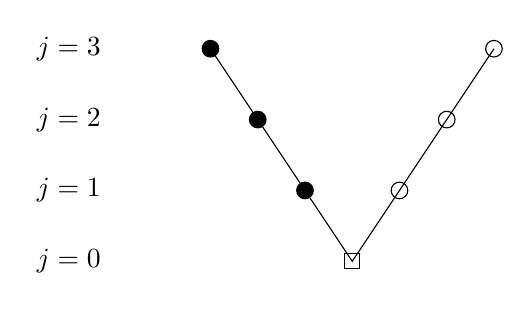
\begin{tikzpicture}[scale=1.2]
  \pgfmathsetmacro\hstep{0.5}
  \pgfmathsetmacro\vstep{0.75}
  \pgfmathsetmacro\ceps{0.08}   % size of square for coarse grid

% grid labels at left
  \node at (-2,3*\vstep) {$j=3$};
  \node at (-2,2*\vstep) {$j=2$};
  \node at (-2,\vstep) {$j=1$};
  \node at (-2,0.0) {$j=0$};

% V-cycle
  \draw[black,thin] (-\hstep,3*\vstep) -- (0.0,2*\vstep) -- (\hstep,\vstep) --  (2*\hstep,0.0)
                    -- (3*\hstep,\vstep) -- (4*\hstep,2*\vstep) -- (5*\hstep,3*\vstep);
  \filldraw (-\hstep,3*\vstep) circle (2.5pt);
  \filldraw (0.0,2*\vstep) circle (2.5pt);
  \filldraw (\hstep,\vstep) circle (2.5pt);
  \draw     (2*\hstep-\ceps,-\ceps) rectangle (2*\hstep+\ceps,+\ceps);
  \draw     (3*\hstep,\vstep) circle (2.5pt);
  \draw     (4*\hstep,2*\vstep) circle (2.5pt);
  \draw     (5*\hstep,3*\vstep) circle (2.5pt);
\end{tikzpicture}

\caption{A V-cycle on a three-level hierarchy ($K=2$) with a down-smoother (solid dots), up-smoother (circles) and coarse-level solver (square).}
\label{fig:vcycle}
\end{figure}

Two new symbols have appeared, however.  First, the residual is \emph{restricted} onto the next-coarser level by the \emph{canonical restriction operator} $R$ which creates a linear functional on the $k-1$ level from a linear functional $\ell^k$ on the $k$ level:
\begin{equation}
  (R \ell^k)[v] = \ell^k[v] \label{eq:canonicalrestriction}
\end{equation}
for all $v$ in $\mathcal{V}^{k-1}$.  That is, $R \ell^k$ acts on $\mathcal{V}^{k-1}$, but it is really just the same as $\ell^k$.  Next, after the recursive solve on the $k-1$ level the coarse-level error $e^{k-1}$ needs to correct the fine-level iterate $w^k$.  This is done by the \emph{canonical prolongation operator} $P$ acting on a function $z^{k-1}$ in $\mathcal{V}^{k-1}$:
\begin{equation}
  (P z^{k-1})(x) = z^{k-1}(x). \label{eq:canonicalprolongation}
\end{equation}
That is, as with the canonical restriction, the result $P z^{k-1}$ is really just the same as the input function $z^{k-1}$.

Though the operators $R$ and $P$ seem to do nothing, and make no choices, which is the meaning of ``canonical'', in fact they represent computational work because of how we represent functions and functionals on a given level.  That work is entirely contained in the perhaps-forgotten equation \eqref{eq:hatcombination} which describes how to a coarse-level hat function is a linear combination of fine-level hats.  For example, if a fine-level linear functional $\ell^k$ is represented on the computer as a vector of its values $\ell[p] = \ell^k[\psi_p^k]$, then the vector representing the restricted linear functional $R \ell^k$ has values computed via \eqref{eq:hatcombination}.  Likewise, if a coarse-level function $z^{k-1}(x)$ is represented by its coefficients in the basis $\{\psi_p^{k-1}\}$ then \eqref{eq:hatcombination} determines the coeffients of $P z^{k-1}$ in the fine-level basis of hat functions $\{\psi_p^k\}$.  As $R$ and $P$ are linear operators, they may of course be represented as rectangular matrices, but this is not at all necessary.  In any case the application of $R$ and $P$ requires $O(m_k)$ work.

The above \textsc{vcycle} algorithm also calls a coarse solver on the $k=0$ level.  For a linear problem like our current Poisson problem it is traditional to apply a direct solver for this linear system (i.e.~equation \eqref{eq:linearsystem}), but again this will not be an option for the nonlinear glacier geometry problem.  Instead we define \textsc{coarsesolve} as the application of a fixed number of GS sweeps.  If the coarsest mesh has a single node then a single sweep suffices to give an exact solution of the $k=0$ problem.
%\begin{pseudo*}
%\pr{coarsesolve}(\ell)\text{:} \\+
%    $w=0$ \\
%    for $j=1,\dots,$\id{coarse} \\+
%        \pr{gssweep}(0,w,\ell) \\-
%    return $w$
%\end{pseudo*}

The goal of this section has been to be as clear as possible about the basic geometric multigrid algorithm.  We have taken a particular FE viewpoint, namely the subspace decomposition approach as pioneered by Xu \cite{Xu1992}, an idea which applies both to multilevel and domain-decomposition algorithms.  Now would be the place to put computational results, which would prominently feature the efficiency of the V-cycle algorithm, namely evidence of optimal $O(m_K)$ time to solve the problem, and indeed such results appear in all of our multigrid references \cite{Briggsetal2000,Bueler2021,Elmanetal2014,Trottenbergetal2001}.  However, we forego such easy-to-produce results in favor of introducing the less-trivial ``obstacle'' problem in the next section, which has the essential free-boundary character of the glacier geometry problem.  Computational results will be given at the ends of the next three sections.


\section{Subset decomposition for the classical obstacle problem} \label{sec:obstacle}

The last section is a quick review, based on the simplest Poisson problem, of a ``classical'' geometric multigrid (GMG) method.  Classical GMG is, however, not adequate for the main problem in glaciers, namely how the geometry and velocity of a glacier evolves in response to climatic inputs.  First the glaciers problem is (famously) nonlinear, in that the fluid is non-Newtonian, but this is not the leading difficulty.  Rather, regardless of the manner in which momentum (stress) balance is modeled, the boundary condition for the geometry evolution (i.e.~mass conservation) problem arises from an inequality constraint.  Namely that the ice thickness is nonnegative, equivalently that the ice surface elevation is above the bed elevation, a point already made in the Introduction but actually addressed in the next section.  For now we note that the addition of such an inequality constraint generates a nonlinear problem, even if the differential equation is linear.  In this section we modify the GMG subspace decomposition approach to solve a classical \emph{obstacle} problem, which combines an inequality constraint with a linear differential equation.  Switching the differential equation to the nonlinear SIA model in the next section will be comparatively an easy change; one can say that the dominant nonlinearity is already present in the classical obstacle problem here.

We solve the classical obstacle problem by a \emph{constraint decomposition} \cite{Tai2003} method, which modifies the subspace decomposition to allow an inequality constraint.  FIXME

FIXME cite for multigrid obstacle \cite{BrandtCryer1983,Bueler2021,GraeserKornhuber2009,Jouvetetal2013}; cite for subset decomp \cite{Tai2003}


\section{Multigrid for a shallow-ice mass conservation problem} \label{sec:sia}

FIXME cite for glaciers as obstacle problems \cite{Bueler2016,Bueler2020,Calvoetal2002,JouvetBueler2012}

FIXME for 2D domains the coarse mesh construction needs reconsideration

\section{Multigrid for a Glen-Stokes glacier flow} \label{sec:stokes}

FIXME multigrid already used for Blatter-Pattyn model \cite{BrownSmithAhmadia2013} and for hybrid \cite{Jouvetetal2013}; one goal of this section is to make these approaches more understandable

FIXME we use Schur complement \cite{Bueler2021,Elmanetal2014} and compare it to Vanka monolithic smoother \cite{Farrelletal2019}

\small

\bigskip
\bibliography{review}
\bibliographystyle{siam}

\end{document}
